\documentclass{TUBAFarbeiten}

\usepackage{selinput}
%	\SelectInputMappings{adieresis={ä},germandbls={ß},Euro={¤}}
\usepackage{graphicx}
\usepackage[T1]{fontenc}
\newcommand{\latex}{\LaTeX\xspace}
\usepackage[hidelinks]{hyperref}
\graphicspath{{fragments/}}




\TUBAFFakultaet{Mathematik und Informatik}
\TUBAFTitel{Mensch-Maschine Projekt}
\TUBAFInstitut{Informatik}
\TUBAFUntertitel{Taskanalyse}
\TUBAFAutor{Dennys-Daniel Vogt}
\TUBAFStudiengang{Bachelor Angewandte Informatik}
\TUBAFMatrikel{63411}
\TUBAFDatum{31. August 2021}
\begin{document}
\maketitle
\tableofcontents
\newpage
\TUBAFErklaerungsseite

\section{Theoriefragen}
\subsection{Frage 1: Theorie von Norman}
Die Theorie von Norman ist eine Möglichkeit Probleme im Umgang mit technischen Alltagsgegenständen zu charakterisieren. Diese Charakterisierung unterteilt sich in zwei Unterkategorien, die Kluft der Ausführung und die Kluft der Evaluation.\\
Die Kluft der Ausführung ist der Ausführungsweg des Nutzers mit dem technischen Gerät und unterteilt sich in folgende drei Kategorien:
\begin{enumerate}
	\item Intention (Aktion mit Gerät)
	\item Handlungsplanung (Planung der physischen Handlung)
	\item Ausführung (Ausführung der geplanten Aktion)
\end{enumerate}
Die Kluft der Evaluation ist der Bewertungsweg und unterteilt sich in folgende drei Kategorien:
\begin{enumerate}
	\item Wahrnehmung (System im richtigen Zustand)
	\item Interpretation (Zustand interpretierbar)
	\item Bewertung (Vergleich mit dem Ziel des Nutzers)
\end{enumerate}

\hfill \break
Am Beispiel einer modernen Kaffeemaschine wird die Theorie von Norman nochmals erläutert.

\begin{table}
	\centering
	\caption{Theorie von Norman am Beispiel Kaffeemaschine}
	\begin{tabular}{ll}
		0. Zielsetzung & Erstellung eines Latte Macchiatos\\
		1. Intention & Ist die Maschine fähig diesen Kaffee zu erstellen?\\
		2. Handlungsplanung & Finden des Bildchens mit dem Latte Macchiato\\
		3. Ausführung & Auf das Bildchen drücken\\
		4. Wahrnehmung & Fängt die Maschine an den Kaffee zu erstellen?\\
		5. Interpretation & der Kaffee läuft, alles läuft nach Plan\\
		6. Bewertung & ist am Ende ein Latte Macchiato entstanden oder ein Kuchen?\\
	\end{tabular}
\end{table}


\subsection{Frage 2: ACT-Theorie}
Die ACT-Theorie (eng. Adaptive Control of Thought) beschreibt die Aneignung von Fähigkeiten und ihrer Umsetzung. Das Ziel dieser Theorie ist es das Verhalten des Nutzers zu simulieren. Damit kann man sehen wie schnell ein Nutzer z.B. das Bedienen einer Software erlernen kann. 
Durch die Theorie kann eine potentielle Lernkurve erstellt werden. Bei einer zu steilen Kurve kann entweder die Software vereinfacht werden oder die Dokumentation der Software verbessert werden, um diese abzuflachen.\\

Als Beispiel nehmen wir das Nutzen von \LaTeX\ zur Erstellung von Studienarbeiten. Zuerst werden Fakten, Konzepte und Zusammenhänge durch den Übungsleiter oder durch hilfreiche Websites wie overleaf.com vermittelt. Wenn diese Fakten ausreichend verarbeitet wurden, gelangen diese ins Langzeitgedächtnis. Dieser Teil des Langzeitgedächtnis wird auch als deklaratives Gedächtnis bezeichnet.\\
Das Wissen über Konzepte reicht leider oftmals nicht aus. Um diese auch vollständig implementieren zu können, braucht man Übung. Durch das mehrfache wiederholen von Tabellenerstellung in \LaTeX\ und das ständige Anpassen an den gegebenen Inhalten und Umständen, wird dies automatisiert und kann folglich auf fast jede weitere Aufgabe angewandt werden.
Diesen Teil des Langzeitgedächtnises nennt man Produktionsgedächtnis.\\

Erhält man eine neue Aufgabe (Erstellung einer Tabelle) mit wieder neuen Kriterien und Daten wird im Arbeitsgedächtnis auf das deklarativen Gedächtnis zugegriffen um die Grundlagen (Konzepte, Begriffe, etc.) zu nutzen und auf das Produktionsgedächtnis um die bereits ausgeführten Erfahrungen auf das neue Beispiel anwenden zu können. \\

Die ACT-Theorie kann wesentliche Phänomene des
Lernens erklären. Diese kann die veränderte Denkweise des Nutzers vom Anfänger bis zum Experten darstellen. Am Anfang der Tabellenerstellung dauerte es noch sehr lange bis die Tabelle vollständig implementiert wurde und als Experte dauert es nur noch Sekunden. Unter anderem werden somit auch Gewohnheiten gebildet, die zur schnelleren Ausführung hilfreich sind.  

\subsection{Frage 3: Fehlervermeidung durch Benutzer}
Fehler sind täglich vorprogrammiert und der Benutzer wird immer Fehler machen. Diese Fehler können aber teilweise vermieden werden. Eine aussagekräftige Fehlermeldung ist ein Beispiel um diese künftig zu vermeiden. Als Beispiel dient wieder \LaTeX. Es ist deutlich hilfreicher wenn in den Fehlermeldungen beim kompilieren nicht \glqq Syntaxfehler\grqq{} steht sondern \glqq der Table Block wurde nicht geschlossen\grqq{}. \\
Ein übersichtliches Layout ist ebenfalls hilfreich um Fehler eines Nutzers zu vermeiden. Eine kleine Beschreibung beim hovern über Symbole als auch die Übersichtlichkeit in der Taskleiste von \LaTeX\ hilft den Nutzer nicht willkürlich irgendwelche Knöpfe zu drücken, die nicht zum gewünschten Ziel führen. \\
Sehr viele Fehler entstehen bei einer multilingualen Bedienung. Wenn das ganze Programm auf Englisch ist und der Nutzer kein Englisch versteht können viele Fehler entstehen. Ob es durch Google Translator ist oder durch das Ausprobieren der Funktionen bis eine funktioniert und das Macht was man möchte. \LaTeX\ kommt glücklicherweise in mehreren Sprachen, obwohl die Kommandos trotzdem in Englisch bleiben. \\
Die Sprache ist ebenfalls Teil der Konsistenz. Dabei sollte man darauf achten, dass die Terminologie dann auf die ausgewählte Sprache angepasst ist. Natürlich gibt es auch \glqq eingedeutschte\grqq{} Begriffe aber das Ganze muss stimmen. Ebenfalls fällt in die Konsistenz die Struktur, Darstellung und Interaktionsmöglichkeiten hinein. Hierbei sind Beispiele die Anordnung von Symbolen, das Farbschema des Programms oder das Verhalten der Maustasten. \\
Der Nutzer sollte einen leichten Einstieg in die Software haben. Wenn diese aber von Natur aus schon komplex ist, sollte eine ausreichende Dokumentation oder ein Kurs dazu erstellt werden. \\
Im Grunde sollte man sich stets Gedanken machen welche Nutzer die Software nutzen werden. Dazu könnte man entsprechende Personas bilden um die Aufgaben und Ziele der einzelnen Benutzergruppen zu identifizieren.

\newpage
\subsection{Frage 4: Arbeitsgedächtnis unterstützen}
Das Arbeitsgedächtnis ist ein wichtiger Teil des Gehirns, der Kombinationen und Verknüpfungen im Moment erstellen kann. Bis vor kurzem wurde angenommen, dass ein Mensch ca. 7 Einheiten gleichzeitig im Arbeitsgedächtnis verarbeiten kann. Neuere Studien besagen, dass diese Zahl bei 3-4 Einheiten liegt und damit deutlich kleiner ausfällt. Um den Arbeitsprozess zu vereinfachen kann man diese Einheiten auch als Chunks bezeichnen. Chunking kommt aus dem englischen und bedeutet so viel wie Bündelung. Somit besagt das Chunking indem wir Einheiten Bündeln und logisch Verknüpfen ist es uns leichter diese Daten zu verarbeiten oder zu merken. Als Beispiel könnte eine Anreihung von Buchstaben dienen. Um sich diese besser merken zu können, könnte man diese auf Wörter aufteilen. Somit macht dies deutlich mehr Sinn. Um dies eine weitere Ebene zu abstrahieren könnte man diese Wörter zu einem Satz zusammen fassen. Somit hat man aus einem sehr schwer zu verarbeitenden Chunk (Aneinanderreihung von Buchstaben) in mehrere kleine Chunks (Wörter) und dann zu einem wieder größeren aber deutlich verständlicheren Chunk (Satz) verwandelt. \\
Bezogen auf die getestete Software wurde dies äußerst gut umgesetzt. Statt umständlicher Namen der Roboter wurden Bilder verwendet. Im Kreismenü wurden ebenfalls Bilder genutzt statt Wörter. Die Menütätigkeiten wurden auch im Bezug auf Chunking implementiert, somit konnte man schnell und einfach durch das Kreismenü navigieren und war nie mit zu vielen Chunks überfordert. Eine konkrete Erweiterung fällt mir dazu nicht ein.

\subsection{Frage 5: Affordanz und Feedback}
Affordanzen werden auch Angebotscharakter oder angebotene Gebrauchseigenschaft genannt. Die angebotene Gebrauchseigenschaft beschreibt die Definition recht gut. Dabei werden zwei Eigenschaften in Beziehung gesetzt und deren mögliche Aktionen ebenfalls. Ein schlechtes Beispiel für Affordanzen im Alltag sind Norman Türen (eng. Norman Doors). Bei diesen wird sinnlich durch das Design vermittelt, dass man ziehen/drücken müsste, um eine Tür zu öffnen aber ein Schild daneben sagt das komplette Gegenteil aus. Eine Darstellung solch einer Norman Tür  ist in Abbildung \ref{fig:norman} zu sehen. 

\begin{figure}
	\centering
	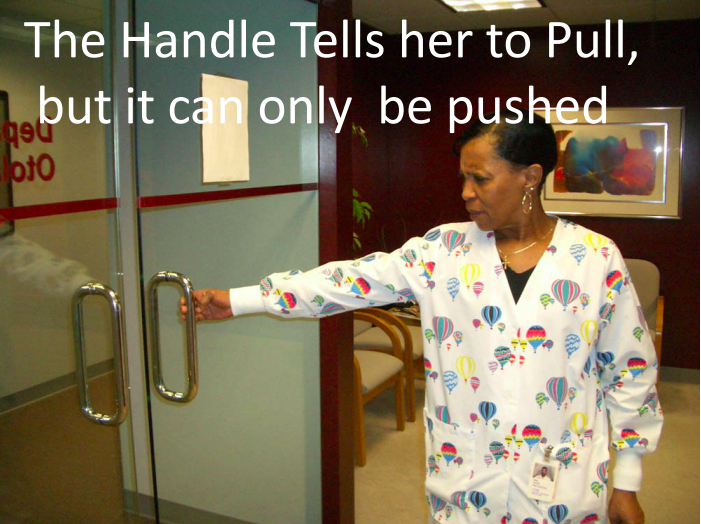
\includegraphics[width=10cm]{norman.png}
	\caption{Norman Tür}
	\label{fig:norman}
\end{figure}

Bei Betrachtung der Testsoftware sind im Bereich der Affordanz das Verhalten und Nutzen der physischen Knöpfe zu beachten. 
Aber auch auf UI-Objekten (Buttons, Pop-Ups, Scroll-Bars etc.) ist zu achten. Dabei soll es nachvollziehbar sein, welchen Sinn ein Objekt hat. Zum Beispiel wird ein physischer Knopf zum Drücken genutzt, aber auch ein Button. Werden diese intuitiven Funktionen auch korrekt genutzt?

Feedback (eng. Rückmeldung) ist eine Möglichkeit den Entwicklern von Software Testinformationen über ihre Software zukommen zu lassen. Dabei wird beachtet, ob diese sich ordnungsgemäß verhält. In diesem Prozess werden Bugs entdeckt, Fehler behoben oder ein Lob ausgesprochen, was zur Weiterentwicklung oder Vollendung der Software beiträgt.

Affordanz und Feedback ist in Kombination sehr mächtig. Mit der Affordanz werden die Missstände in der Software aufgeklärt und durch das Feedback werden diese Informationen an die Entwickler weitergegeben. Eine Verbesserung der Software wird dadurch angetrieben.

\newpage
\section{Projektzusammenfassung}
Das Projekt wurde in fünf Punkte unterteilt. Diese sind Taskanalyse, Personas, Menüentwurf, Testdurchführung und zuletzt die Evaluation. In der Taskanalyse wurden die Toplevel-Tasks identifiziert und konkretisiert. Das Ziel der Taskanalyse war es häufig genutzte Funktionen einfach und schnell zugänglich zu machen. Dazu wurden Toplevel-Tasks und deren Sub-Tasks definiert. 

Die Personas beschäftigten sich mit der Identifizierung der Zielgruppen (z.B.Studenten, wissenschaftl. Mitarbeiter, externe Nutzer). Dabei wurden 8 Personas (2x Studenten, 3x Mitarbeiter, 3x Externe) erstellt. Zusätzlich wurden Besonderheiten der Personen wie Einschränkungen mit implementiert, um die Software auf Benutzerfreundlichkeit dieser eingeschränkten Personen zu bewerten.

Der Menüentwurf beschäftigte sich mit der Aufteilung des Menüs in Unterpunkte, um die von der Taskanalyse behandelten Tasks in das Menü effizient einzubinden. 

Die Testdurchführung hat die Software auf die Toplevel-Tasks getestet. Ebenfalls wurde auf die Besonderheiten der Personas eingegangen. Ebenfalls wurde ein Vergleich des realen Menüs mit dem Menüentwurf gestaltet und dieses wurde auf Effizienz getestet. Die gesammelten Informationen wurden an die Evaluation weitergegeben.

Die Evaluation hat die bereits vorhandenen Daten aus den vorherigen Teilen aufgearbeitet und in Schemata dargestellt. Dazu wurden Kriterien bestimmt, um die Begutachtung und Gebrauchsfähigkeit der Anwendung zu evaluieren. Diese Kriterien werden auch Heuristiken genannt.\\

Mein persönlicher Eindruck und Informationen, die ich aus diesem Projekt mitgenommen habe sind recht zwiegespalten. Einerseits war es eine Interessante Erfahrung mit teils neuen Leuten an einem Projekt zu arbeiten und sich in ein Thema einzuarbeiten. Ebenfalls gab es viele neue Erkenntnisse im Bereich UI/UX und man konnte den ganzen Prozess nachvollziehen und begutachten. Dies ist auch hilfreich für die künftige Berufswahl. Leider gab es auch negative Aspekte an dem Projekt. Teilweise war es schwer mit einigen Mitgliedern einen Kommunikationsweg zu finden und die Möglichkeit der Absprache gestaltete sich schwierig. Zusätzlich sind im Laufe des Projekts zwei Teammitglieder abgesprungen und somit ist viel aus unseren 3-Personen-Testdurchführungsteam an einer Person hängen geblieben.\\

Positiv ist mir in Erinnerung geblieben wie Umfangreich und doch detailliert (Softwaretechnisch) die Software aufgebaut war. Viele Funktionen, die vorab in der Taskanalyse besprochen wurden, waren auch implementiert. Der Menüaufbau war übersichtlich und die Shortcuts fürs Wechseln der Transportart waren hilfreich. Zusätzlich ist die Simulation von Fahrenden Robotern und die Pfadplanung interessant erschienen. \\
Zu den negativen Erfahrungen zähle ich die häufigen Bugs. Absolut inakzeptabel war, dass man sich durch zu schnelles Bewegen auf den Kopf stellen konnte. Da wurde mir sogar ohne VR-Brille schlecht. Auch das die (automatische) Pfadplanung der Roboter manchmal nicht optimal läuft und diese sich an kleinen Gegenständen wie Büschen oder an Seiten von Gebäuden festfahren. Ein großer Kritikpunkt für mich war die visuelle Unübersichtlichkeit des Menüs. Die sich bewegenden Wolken im Hintergrund sahen zwar nett aus, aber man konnte oftmals die Schrift der Menüpunkte somit nicht mehr lesen.\\
Das beeindruckendste war, dass diese Software von einer Person im Rahmen einer Bachelorarbeit erstellt wurde.  
 


\newpage
\section{Aufgabenspezifische Fragen: Taskanalyse}
\subsection{Frage 1}
Im folgenden Teil wird die Taskanalyse näher betrachtet. Dazu wird die Darstellung der Top- und Sub-level Tasks genutzt. In der Abbildung \ref{fig:toplevel} werden die sechs Topleveltasks gezeigt. Genutzt wurden diese Tasks, da sie kleinere Tasks vereinen. All diese sind wichtig mit ihren Subtasks.\\\\

\begin{figure}
	\centering
	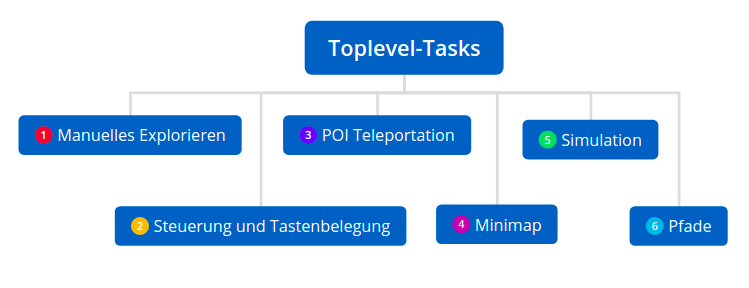
\includegraphics[width=\linewidth]{topleveltask.png}
	\caption{Toplevel-Tasks}
	\label{fig:toplevel}
\end{figure}

Unter dem manuellen Explorieren versteht man die Möglichkeit sich per Kurzdistanz-Teleport, fliegend oder zu Fuß zu bewegen. Dies muss auch einstellbar sein und da der Wechsel oft genutzt wird auch in wenigen Handgriffen oder Klicks umstellbar sein. Zur Veranschaulichung diesen Aspekts siehe Abbildung \ref{fig:explo}.\\

\begin{figure}
	\centering
	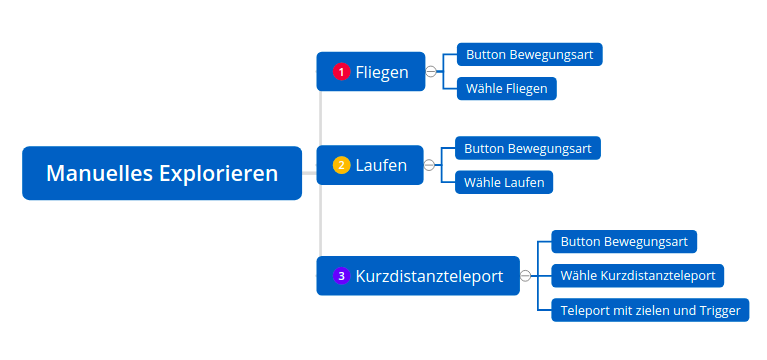
\includegraphics[width=\linewidth]{explorer.png}
	\caption{Manuelles Explorieren}
	\label{fig:explo}
\end{figure}

Die Steuerung und Tastenbelegung ist essenziell um wichtige Aspekte des Programms verändern zu können. Unter diesem Teil fallen viele Untertasks an. In Abbildung \ref{fig:s&t} ist dies zu sehen.

\begin{figure}
	\centering
	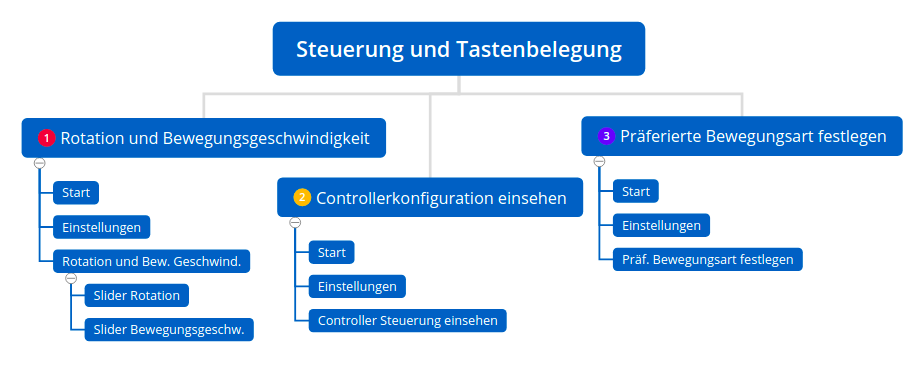
\includegraphics[width=\linewidth]{einstellungen.png}
	\caption{Steuerung und Tastenbelegung}
	\label{fig:s&t}
\end{figure}

Der Task Teleportation zu POI (kurz für Points of Interest) ist ein kleiner aber wichtiger Task. Dieser ermöglicht die Schnellreise in dem Programm um Zeit des Nutzers zu sparen, statt sich zu diesen Ort über die präferierte Bewegungsart hin zu bewegen. In Abbildung \ref{fig:POI} ist dies in einer Grafik dargestellt.

\begin{figure}
	\centering
	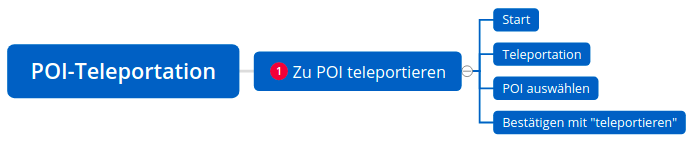
\includegraphics[width=\linewidth]{POI.png}
	\caption{POI Teleportation}
	\label{fig:POI}
\end{figure}

Die Minimap ist zur Orientierung wichtig, dennoch kann sie äußerst störend sein, wenn sie direkt an der VR-Brille klebt. Deswegen ist es notwendig die Position der Minimap ändern zu können oder sogar ganz auszuschalten. Ein weiterer zu implementierender Task wäre die Skalierung der Minimap. Eine kleinere Minimap ist leichter zu betrachten. In Abbildung \ref{fig:mini} ist dies dargestellt.\\

\begin{figure}
	\centering
	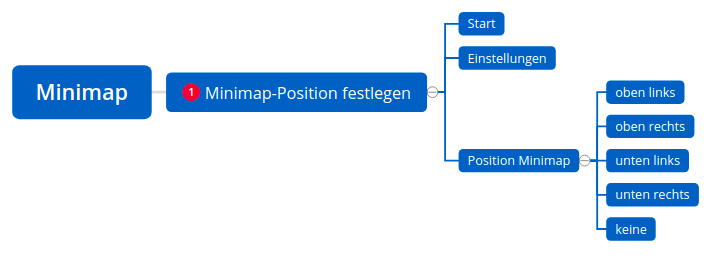
\includegraphics[width=\linewidth]{minimap.png}
	\caption{Minimap}
	\label{fig:mini}
\end{figure}

Unter den Simulationsreiter fallen alles Simulationen von Robotern. Hier sind Tasks aus der Pfadplanung nicht inbegriffen (siehe Pfade Abb. \ref{fig:Pfad}). Um ein besseres Verständnis über die Tasks zu erhalten, die in der Simulation inbegriffen sind, siehe Abbildung \ref{fig:Sim}.\\

\begin{figure}
	\centering
	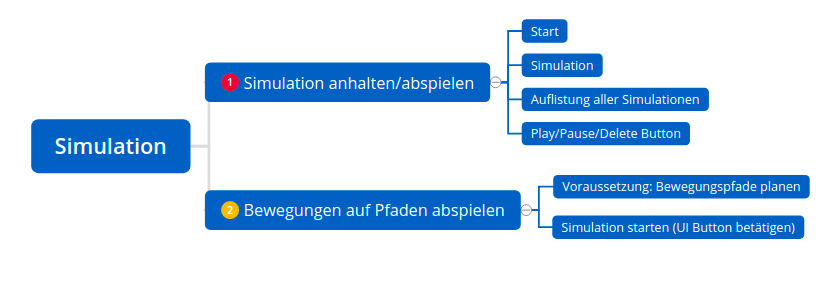
\includegraphics[width=\linewidth]{sim.png}
	\caption{Simulationen}
	\label{fig:Sim}
\end{figure}

Die Pfadplanung ist Voraussetzung für die Simulation. Wenn kein Pfad existiert bewegt der Roboter sich nicht. Man könnte auch das Autolaufen (automatische Bewegen des Spielers zu einen Punkt) aktivieren. In Abbildung \ref{fig:Pfad} ist die Möglichkeit der Pfaderstellung dargestellt. Hierbei kann die Option Simulieren gewählt werden und man würde auf die Simulationsseite mit den vorhandenen Pfad weitergeleitet werden. Hier besteht ebenfalls die Möglichkeit den erstellten Pfad zu exportieren.\\

\begin{figure}
	\centering
	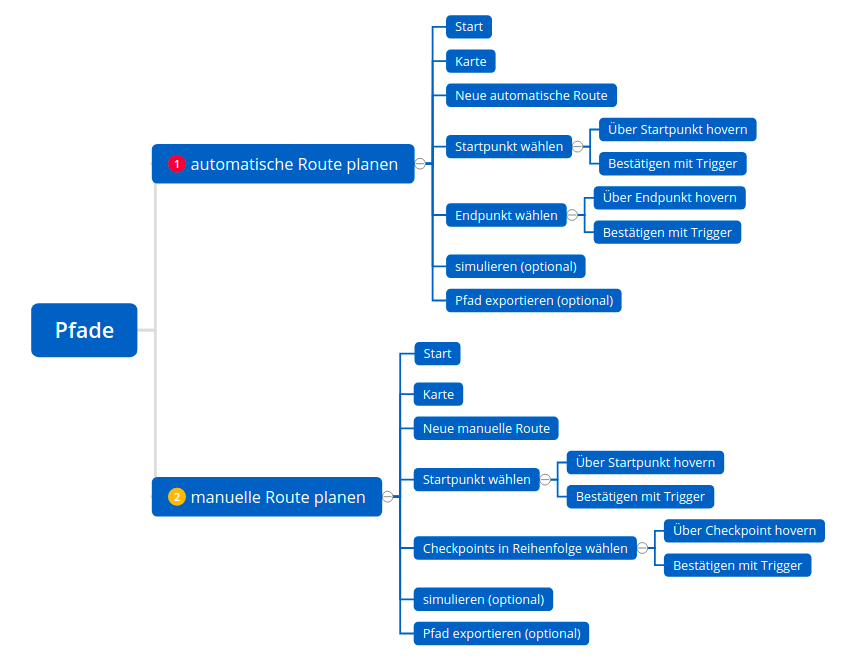
\includegraphics[width=\linewidth]{pfad.png}
	\caption{Pfade}
	\label{fig:Pfad}
\end{figure}

Ich habe diese Aufteilung genutzt um eine Vereinfachung und Übersicht über die Tasks zu schaffen. Deshalb habe ich sie in die Kategorien aus Abbildung \ref{fig:toplevel} aufgeteilt. All diese Kategorien haben Tasks, die essenziell für ein gut laufendes Programm sind. Die Subtasks können eventuell optimiert werden. Zur besseren Darstellungsmöglichkeit habe ich auch für jede einzelne Kategorie ein eigenes Bild erstellt. Dies dient der Übersichtlichkeit.
\newpage
\subsection{Frage 2}
Folgend ist eine geordnete Liste, die meiner Meinung nach die am häufigsten genutzten Tasks enthält.
\begin{enumerate}
	\item Manuelles Explorieren
	\item Bewegungsart ändern
	\item Nutzen des Menüs
	\item Simulationen
\end{enumerate}
In dieser Liste ist das manuelle Explorieren an erster Stelle. Dies liegt daran, dass sich der Spieler kontinuierlich bewegt. Deswegen ist dies meiner Meinung nach der am  häufigsten genutzte Task. Gleich darauf Folgt das Ändern der Bewegungsart. Teilweise zählt das noch zum ersten Punkt, ich wollte es aber nochmals gesondert erwähnen. Das Umstellen der Bewegungsarten wird auch häufig genutzt. Man möchte evtl. im Lauf-Modus nicht langsam unterwegs sein oder durch das schnelle Fliegen wird einem übel, so kann man auf Teleportation umschalten. Das Menü selbst ist kein Task aber ein essenzieller Baustein für fast alle anderen Tasks wie Routenplanung, die Karte, Simulationen etc. Deswegen habe ich dem Menü einen Platz in dieser Liste gegeben. Die Simulation erreicht bei mir Platz vier. Für mich persönlich ist das ein recht irrelevanter Task, aber es kommt drauf an wer die Software verwendet. Wird diese von Robotikern genutzt, spielt die Simulation eine große Rolle. Auch wenn es witzig war mit den Robotern in der Software herum zu spielen.\\

\subsection{Frage 3}
Das folgende Szenario wird in der Software mit Maus und Tastatur getestet.
Dabei handelt es sich um diesen Ablauf:
\begin{enumerate}
	\item Start des Programms
	\item Spawnen am Audimax
	\item Kurzdistanzteleport an eine umliegende Stelle
	\item Route planen nach Tagebautechnikum  
	\item Spawnen eines Roboters
\end{enumerate}
In Abbildung \ref{fig:logic} wird der zeitorientierte Programmablauf dargestellt. Zur Darstellungsmöglichkeit zum logischen oder zeitorientierten Ablauf vergleiche Quelle \cite[S. 80-82]{ISB2}.

\begin{figure}
	\centering
	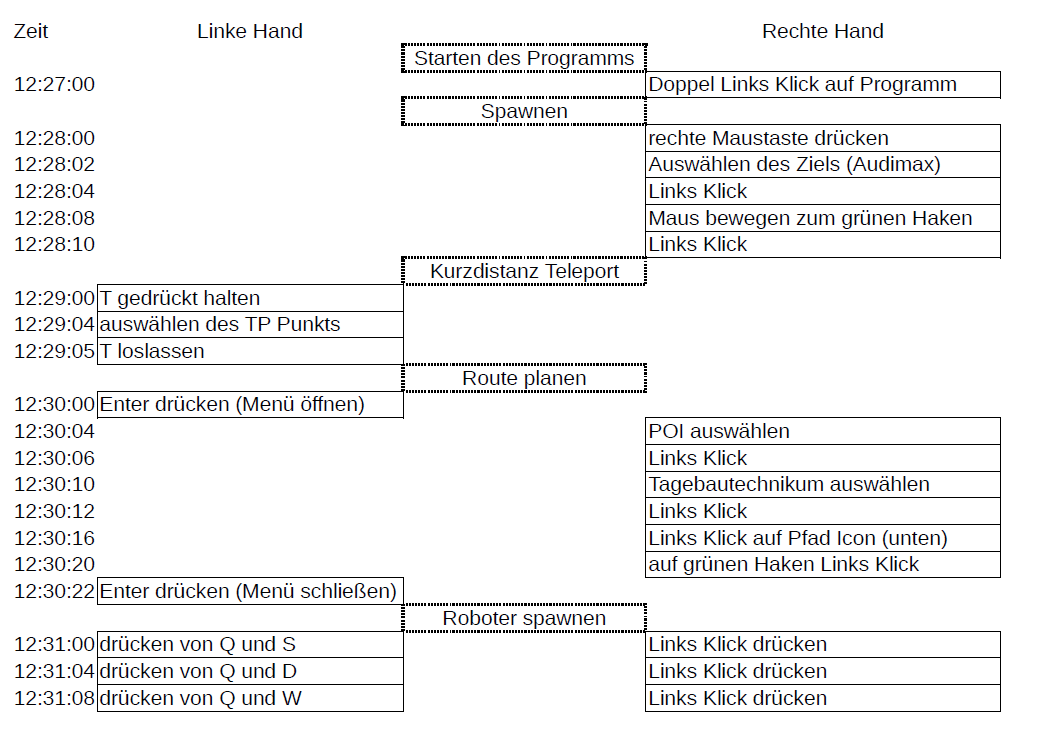
\includegraphics[width=\linewidth]{logic.png}
	\caption{Zeitlicher Ablauf des Szenarios}
	\label{fig:logic}
\end{figure}
\newpage

\subsection{Frage 4}
\label{sec:nichtunterstuetztetask}
In der Testsoftware wurden einige Tasks nicht implementiert. Diese wären:
\begin{itemize}
	\item präferierte Bewegungsart auswählen
	\item Position der Minimap auswählen
	\item Skalierung der Minimap-Größe
	\item Tastenbelegung von Maus und Tastatur einsehen
\end{itemize}
Die o.g. Tasks sind meiner Meinung nach wichtig. Betrachtet wird jeder Einzelne. \\
Die präferierte Bewegungsart auszuwählen ist eine Möglichkeit effizient Zeit zu sparen. Wenn das Laufen die Standardeinstellung ist, ändert sich nichts zum bisherigen Programm. Möchte man aber kontinuierlich fliegen und das Laufen nicht in Betracht ziehen, ist es hilfreich dies auswählen zu können. Das gleiche zählt auch für den Kurzdistanzteleport. Falls der User unter Motionsickness leidet und die Teleportation die einzige Möglichkeit ist das Programm zu nutzen, wäre es vorteilhaft nicht kontinuierlich die T-Taste drücken zu müssen.\\
Die Position der Minimap ist standardmäßig in der unteren rechten Ecke zu finden. Diese kann auch ausgeschaltet werden. Nur leider kann man nicht die Position ändern. Es wäre schön die Auswahl zu haben in welche der Ecken die Karte erscheinen soll.\\
Wenn die Minimap angeschaltet ist, nimmt diese einen sehr großen Platz ein. Meiner Meinung nach ist die aktuelle Größe der Minimap schon zu groß. Hier wäre es schön die Größe der Minimap mit z.B. einen Slider ändern zu können. Gefühlt nimmt die Minimap 20\% des Bildschirms ein. 
\subsection{Frage 5}
Ich würde die Nutzer selbst fragen, um herauszufinden, welche Tasks noch benötigt werden. Ein Test wäre von Vorteil. Hier werden nicht nur Bugs entdeckt, sondern evtl. werden von den künftigen Nutzern auch Tasks gewünscht, die noch nicht implementiert wurden. Als Entwickler ist man oftmals in einer Bubble und kann nicht genau über die eigene Software urteilen. Dadurch ist es sehr hilfreich von Anfang an den Nutzer mit zu integrieren.
\subsection{Frage 6}
Es gibt einige Tasks, die für Akzeptanz bei den Nutzern sorgen. Das manuelle explorieren ist einer dieser Tasks. Hier ist zu beachten, dass ohne diesen Task die ganze Software sinnlos wäre. Der Task sollte aus diesen Grund ohne Probleme funktionieren. Je nach Anwendungsbereich kommt die Simulation von Robotern und die Pfadplanung dazu. Aus Sicht eines Robotikers ist dies der primäre Task und äußerst wichtig. Als letztes würde ich noch die Funktion der Weltgenerierung betrachten. Hierbei handelt es sich nicht um einen Task, aber die Simulation der Umgebung ist wichtig für z.B. die Simulation der Roboter.\\
Um eine Steigerung der Effizienz eines Nutzers zu erlangen, gibt es nach meiner Meinung nur einen Task: Die präferierte Bewegungsart auswählen. Wie in Kapitel \ref{sec:nichtunterstuetztetask} bereits erläutert, ist eine zeitliche Einsparung möglich und dies führt somit zu einer erhöhten Effizienz.


\newpage
\listoffigures
\newpage
\listoftables
\newpage
\bibliography{mmk.bib}
\bibliographystyle{IEEEtran}
\end{document}